\documentclass{article}
\usepackage[utf8]{inputenc}
\usepackage[spanish]{babel}
\usepackage{listings}
\usepackage{graphicx}
\graphicspath{ {images/} }
\usepackage{cite}

\begin{document}

\begin{titlepage}
    \begin{center}
        \vspace*{1cm}
            
        \Huge
        \textbf{Desafío de objetos}
            
        \vspace{0.5cm}
        \LARGE
            
            
        \vspace{1.5cm}
            
        \textbf{Ferney Mejía Pérez}
            
        \vfill
            
        \vspace{0.8cm}
            
        \Large
        Departamento de Ingeniería Electrónica y Telecomunicaciones\\
        Universidad de Antioquia\\
        Caldas-Antioquia\\
        Marzo de 2021
            
    \end{center}
\end{titlepage}

\tableofcontents
\newpage
\section{Sección introductoria}\label{intro}
El objetivo principal de este trabajo es la realización y ejecución de una actividad propuesta por el docente guía del curso en proceso de Informática II, el cual está compuesto por un ejercicio inicial que hace énfasis en la descripción detallada de la traslación de un objeto ubicado en un punto A a un punto B. Además, tras realizar dicha actividad, se presenta la solución del problema mediante instrucciones a tres personas comunes con el fin de poner a prueba cuán óptimo y cuán comprensible es el resultado de dicho proceso.


\section{Sección de contenido} \label{contenido}
A continuación, se presentan cuatro secciones, en las cuales se describen el problema, la solución a este recurriendo a instrucciones, también, se expone el problema y la solución mediante imágenes, y por último, se adjunta un link al sitio web que almacena un vídeo que contiene el experimento con tres personas voluntarias dispuestas a poner en prueba la efectividad de dichas instrucciones.

\subsection{Problema}
Se tienen tres elementos que se presentan en la sección \ref{imagenes}, los cuales serán implementados para plantear el problema como tal.
Ahora bien, la condición inicial es la siguiente; se debe hacer uso de una superficie plana (mesa), en la cuál tras ubicar las tarjetas de igual tamaño y proporción por debajo de la hoja en blanco sobre dicha superficie, se debe proceder haciendo uso de sólo una mano, a tratar de formar una pirámide como se indica en la figura \ref{fig:Piramide}.

\subsection{Instrucciones de solución}
1. Si la hoja en blanco está ubicada en posición vertical, girarla hasta que quede ubicada en posición horizontal.

2. Si la hoja está ubicada en posición horizontal omitir el paso 1.

3. Por condiciones naturales al posicionar de forma horizontal la hoja se forma un rectángulo. Ahora bien, hacer un doblez en la parte superior del ancho del rectángulo hasta la mitad de la hoja. Repetir el proceso pero en la parte inferior del ancho del rectángulo. 

4. Por consiguiente, se presencia que la nueva forma de la hoja queda de manera similar a un plegable. Levantar la hoja desde cualquier parte tratando de mantener dicha forma, desplazarla unos cuantos centímetros a la derecha hasta ver que se puedan presenciar las tarjetas y descargarla sobre la misma superficie plana inicial (mesa).

5. Si las tarjetas se encuentran desordenadas o regadas, sobreponer una ante la otra, levantarlas y desplazarlas unos centímetros a la izquierda de la superficie plana inicial y descargarlas. 

6. Ahora, volver a sujetar la hoja en blanco manteniendo la forma del plegable y levantarla para ubicarla en la posición inicial sobre la superficie plana (mesa) de la cuál fue desplazada. Cabe anotar que, la posición de la hoja debe ser exactamente igual al momento en que fue retirada por primera vez, es decir, ubicar la hoja de forma horizontal (estado inicial en forma de plegable). Luego girar la hoja hacia arriba (90°) hasta quedar de forma vertical. 

7. Dirigirse hacia las tarjetas que deben estar sobrepuestas, sujetarlas con las yemas de los dedos manteniendo la sobreposición, luego, levantarlas.

8. Después de levantar las tarjetas sobrepuestas, girar las tarjetas de manera horizontal hasta formar un rectángulo pequeño. Si se repara en la posición de las tarjetas y la hoja, se forma un eje coordenado (x,y).

9. Teniendo en cuenta esa imagen mental del eje coordenado (x,y), tratar de ubicar las tarjetas sobre el centro de la hoja (origen del eje) y apoyarlas sobre esta.

10. Levantar el dedo meñique para mayor maniobrabilidad, luego deslizar levemente ambas tarjetas hacia los doblez de las hojas y sin permitir que se desplomen las tarjetas, formar una pirámide como se presencia en la figura \ref{fig:Piramide}.

11. Luego de formar la pirámide, liberar el agarre de la mano a las tarjetas levemente para evitar dañar la figura.

\section{Inclusión de imágenes} \label{imagenes}
\begin{figure}[h]
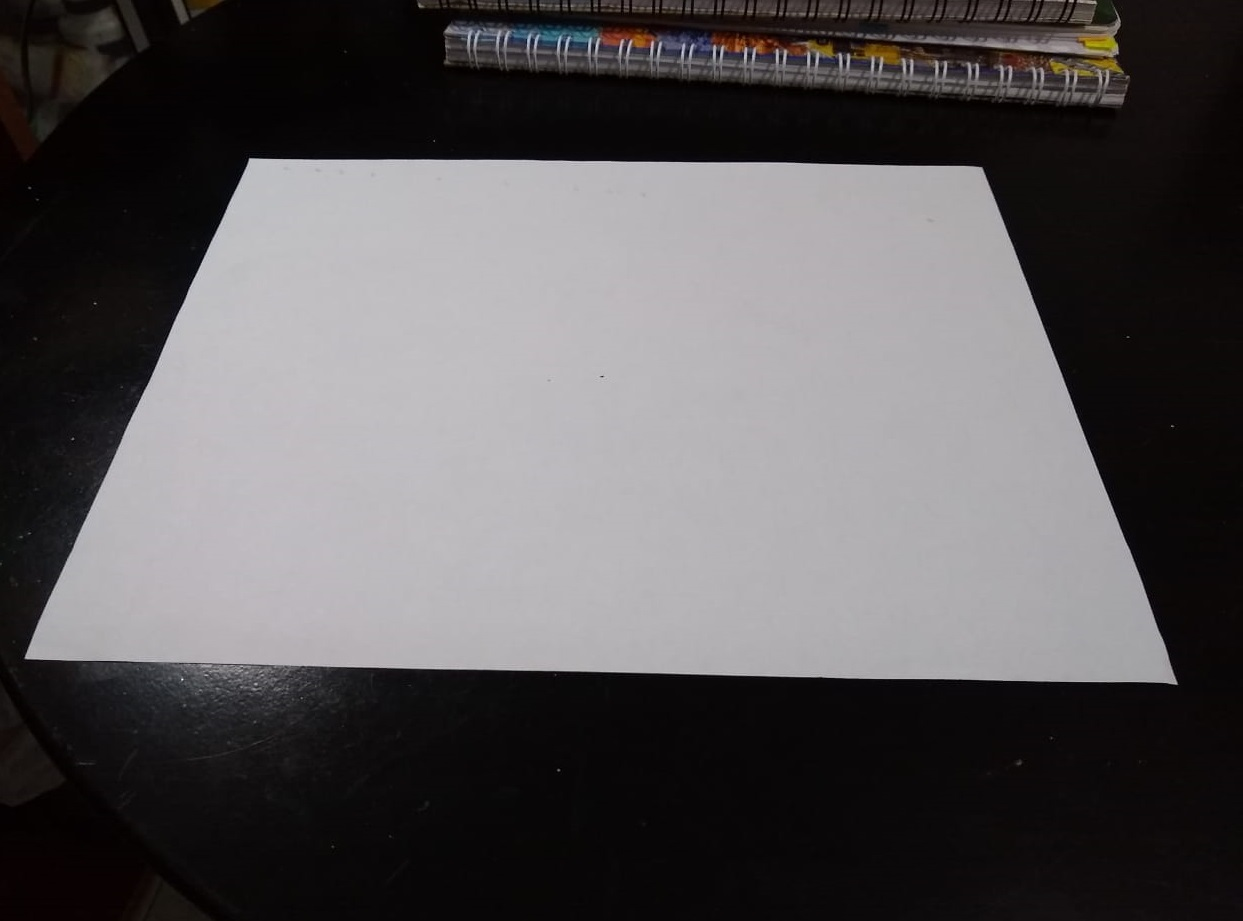
\includegraphics[width=4cm]{Hoja.jpeg}
\centering
\caption{Hoja en blanco}
\label{fig:Hoja}
\end{figure}
\begin{figure}[h]
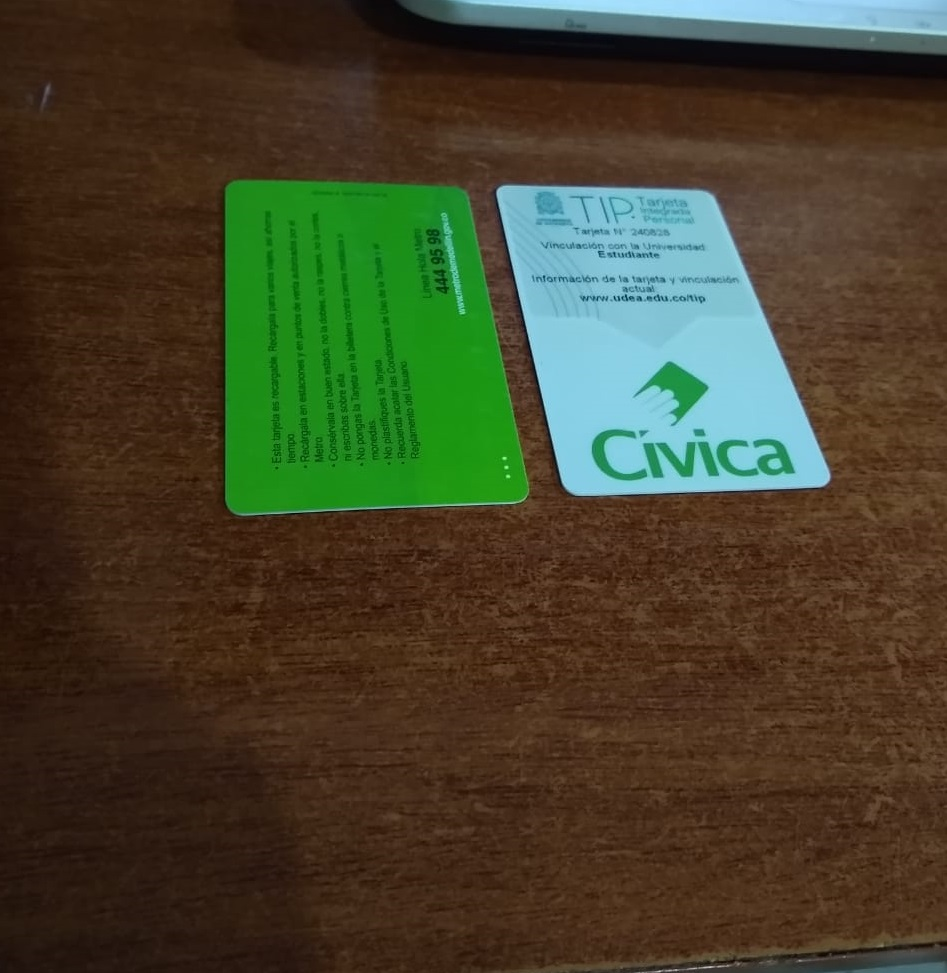
\includegraphics[width=4cm]{Tarjetas.jpeg}
\centering
\caption{Tarjetas de igual tamaño y proporción}
\label{fig:Tarjetas}
\end{figure}
\begin{figure}[h]
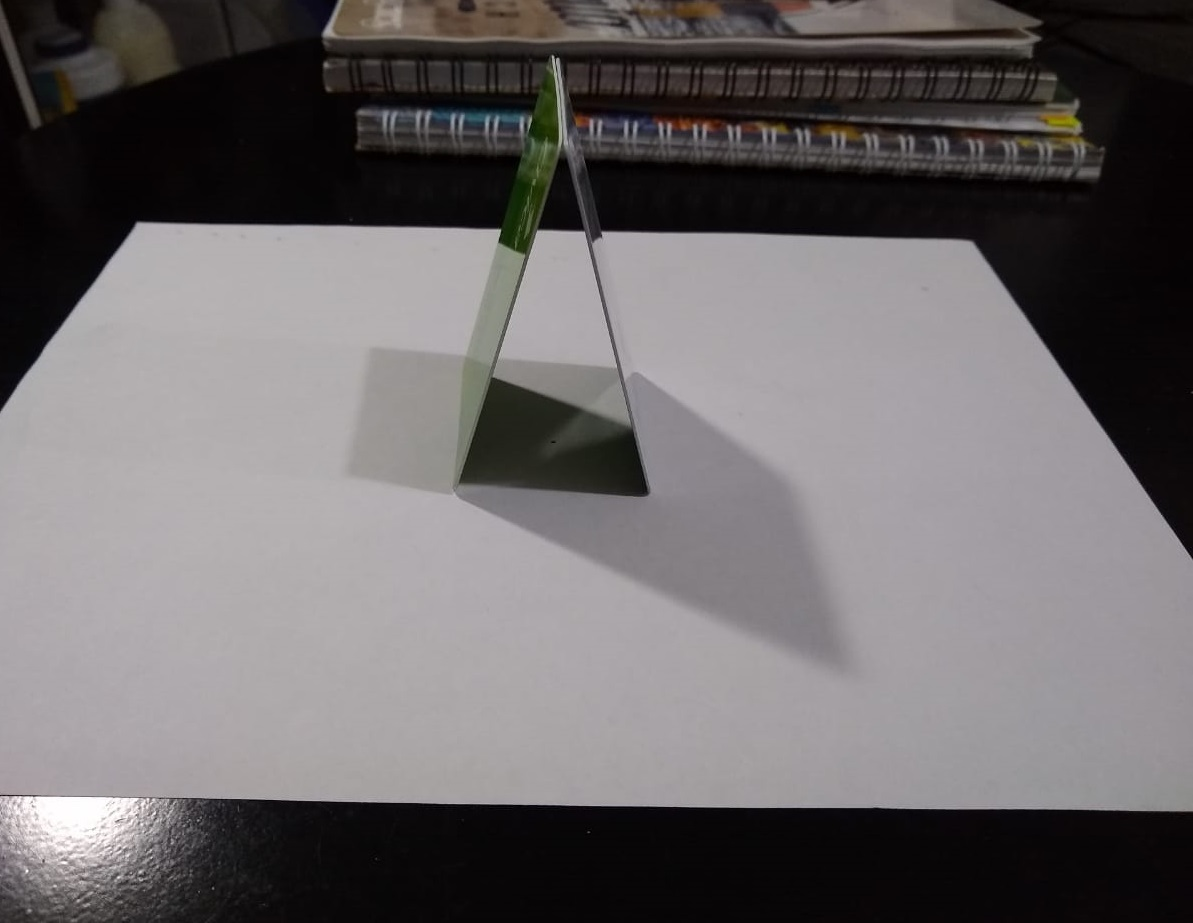
\includegraphics[width=5cm]{Piramide.jpeg}
\centering
\caption{Resultado esperado(pirámide)}
\label{fig:Piramide}
\end{figure}

\section{Link del experimento}
Haciendo uso de la plataforma de YouTube se añade el link del experimento realizado:
\end{document}
